\section{Context Awareness}
Improving the computers ability to access and understand a user's circumstances give developers more information for creating  applications that respond and adapt to the user. A way to accomplish this is to not only use data given by the user, but also use context information from the user's environment. According to Dey in \cite{dey2001understanding}, the definition of context is:

\begin{quotation}
\centering
Context is a combination of any information that can be sensed or received by an entity which is useful to catch events and situations.
\end{quotation}

In other words, context is information from an entity that gives specific information to increase the understanding of an events environment. An entity can be a person, place or an object that is relevant for the interaction. 

One way of generating and sharing this context information on a large scale is through the use of smart telephones and other ubiquitous computing devices. One such smartphone is the a Google Nexus 4 \cite{GoogleNexus} which contains, among other things, an accelerometer to detect acceleration, a GPS to receive location data, a gyroscope to detect rotation, a barometer to detect air pressure and a compass for direction and navigation. By applying sensor fusion \cite{Elmenreich02sensorfusion} other context data can be attained. The phone will collect context-information from its GPS sensor and based on this location be able to give directions. With this extra context information, we can create applications that are context aware. This idea of context awareness is summarized by Dey in \cite{dey2001understanding} as: 

\begin{quotation}
\centering
A system is context-aware if it uses context to provide relevant information and \slash or services to the user, where relevancy depends on the user's task.
\end{quotation}

An example of context-awareness in applications is Google Latitude \cite{GoogleLatitude}, where it's possible to see your friends' location on a map, as shown in figure \ref{googlelat}. Other good examples include applications on smartphones and tablets which rotate the image on screen based on the device's physical orientation as shown in figure \ref{androidorientation}.

\begin{figure}[t] % To force on specific place use H
	\centering
    	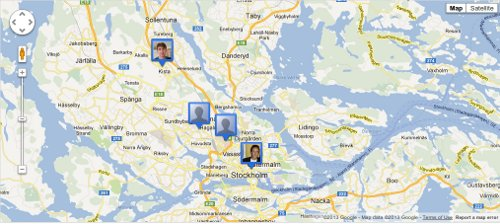
\includegraphics[scale=0.75]{part_2/context_awareness/latitude_pic.jpg}
		\caption{A picture of Google Latitude showing contacts shared positions.} 
		\label{googlelat}
\end{figure}

Context awareness can change classical scenarios into intelligent responsive scenarios by using context information to determine a behavior, such as turning on lights in the house when the user approaches home. Context awareness on a massive scale is gradually enabled by the advances in pervasive and ubiquitous computing.

\begin{figure}[t] % To force on specific place use H
	\centering
    	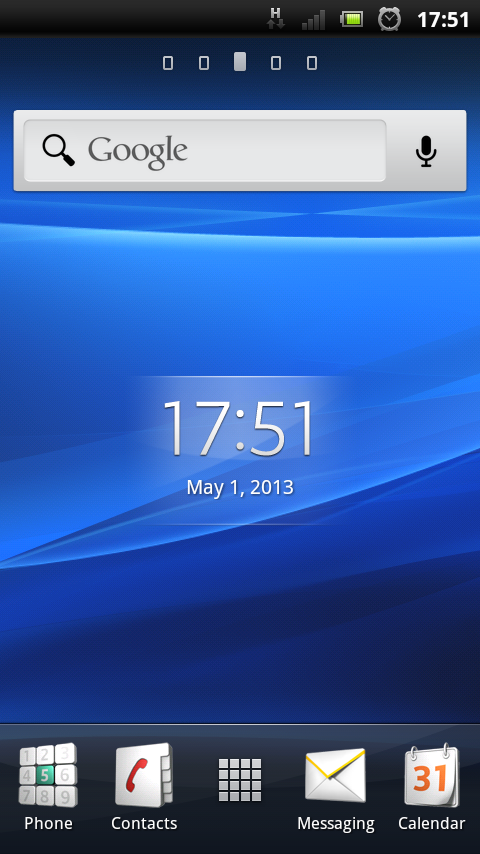
\includegraphics[scale=0.20]{part_2/context_awareness/screenshot_2013-05-01_1751.png}
    	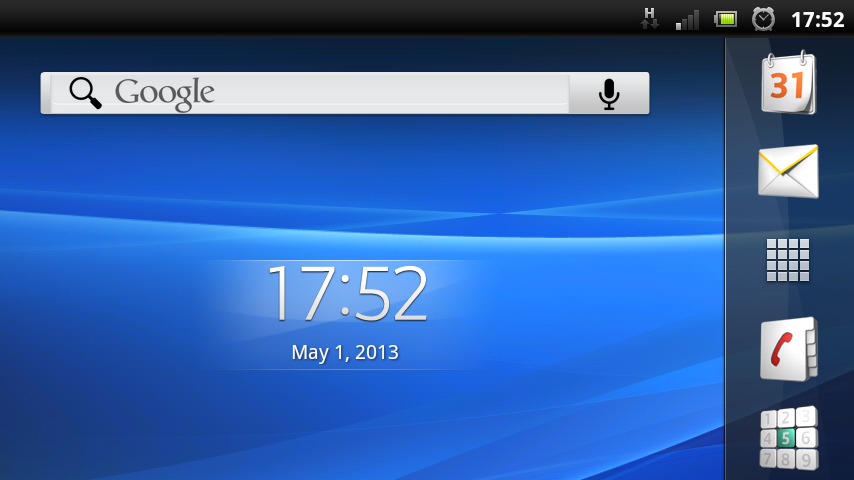
\includegraphics[scale=0.20]{part_2/context_awareness/screenshot_2013-05-01_1752.png}
		\caption{Android homescreen on a Sony Ericsson Xperia PLAY rotates based on context information from its sensors when the phone is 	physically rotated.} 
		\label{androidorientation}
\end{figure}
